%        File: arfc-beamer.tex
%     Created: Sun May 5 10:00 PM 2013 C
%


%\documentclass[11pt,handout]{beamer}
\documentclass[9pt]{beamer}
\usetheme[white]{Illinois}
%\title[short title]{long title}
\title[Short Title]{Useful Practices in Open-Source software development for Nuclear Science and Engineering}
%\subtitle[short subtitle]{long subtitle}
\subtitle[Short SubTitle]{Mostly Kittens}
%\author[short name]{long name}
\author[Your Name]{Oleksandr Yardas\\Advanced Reactors and Fuel Cycles Group}
%\date[short date]{long date}
\date[04.01.2100]{April 16, 2022}
%\institution[short name]{long name}
\institute[UIUC]{University of Illinois at Urbana-Champaign}

%\usepackage{bbding}
\usepackage{amsfonts}
\usepackage{amsmath}
\usepackage{xspace}
\usepackage{graphicx}
\usepackage{subfigure}
\usepackage{booktabs} % nice rules for tables
\usepackage{microtype} % if using PDF
\usepackage{bigints}
\usepackage{minted}

\newcommand{\units}[1] {\:\text{#1}}%
\newcommand{\SN}{S$_N$}%{S$_\text{N}$}%{$S_N$}%
\DeclareMathOperator{\erf}{erf}
%I need some complimentary error funcitons... 
\DeclareMathOperator{\erfc}{erfc}
%Those icons in the references are terrible looking
\setbeamertemplate{bibliography item}[text]

%%%% Acronym support

\usepackage[acronym,toc]{glossaries}
%\newacronym{<++>}{<++>}{<++>}
\newacronym[longplural={metric tons of heavy metal}]{MTHM}{MTHM}{metric ton of heavy metal}
\newacronym{ABM}{ABM}{agent-based modeling}
\newacronym{ACDIS}{ACDIS}{Program in Arms Control \& Domestic and International Security}
\newacronym{AHTR}{AHTR}{Advanced High Temperature Reactor}
\newacronym{ANDRA}{ANDRA}{Agence Nationale pour la gestion des D\'echets RAdioactifs, the French National Agency for Radioactive Waste Management}
\newacronym{ANL}{ANL}{Argonne National Laboratory}
\newacronym{API}{API}{application programming interface}
\newacronym{ARE}{ARE}{Aircraft Reactor Experiment}
\newacronym{ARFC}{ARFC}{Advanced Reactors and Fuel Cycles}
\newacronym{ASME}{ASME}{American Society of Mechanical Engineers}
\newacronym{ATWS}{ATWS}{Anticipated Transient Without Scram}
\newacronym{BDBE}{BDBE}{Beyond Design Basis Event}
\newacronym{BIDS}{BIDS}{Berkeley Institute for Data Science}
\newacronym{CAFCA}{CAFCA}{ Code for Advanced Fuel Cycles Assessment }
\newacronym{CDTN}{CDTN}{Centro de Desenvolvimento da Tecnologia Nuclear}
\newacronym{CEA}{CEA}{Commissariat \`a l'\'Energie Atomique et aux \'Energies Alternatives}
\newacronym{CI}{CI}{continuous integration}
\newacronym{CNEN}{CNEN}{Comiss\~{a}o Nacional de Energia Nuclear}
\newacronym{CNERG}{CNERG}{Computational Nuclear Engineering Research Group}
\newacronym{COSI}{COSI}{Commelini-Sicard}
\newacronym{COTS}{COTS}{commercial, off-the-shelf}
\newacronym{CSNF}{CSNF}{commercial spent nuclear fuel}
\newacronym{CTAH}{CTAHs}{Coiled Tube Air Heaters}
\newacronym{CUBIT}{CUBIT}{CUBIT Geometry and Mesh Generation Toolkit}
\newacronym{CURIE}{CURIE}{Centralized Used Fuel Resource for Information Exchange}
\newacronym{DAG}{DAG}{directed acyclic graph}
\newacronym{DANESS}{DANESS}{Dynamic Analysis of Nuclear Energy System Strategies}
\newacronym{DBE}{DBE}{Design Basis Event}
\newacronym{DESAE}{DESAE}{Dynamic Analysis of Nuclear Energy Systems Strategies}
\newacronym{DHS}{DHS}{Department of Homeland Security}
\newacronym{DOE}{DOE}{Department of Energy}
\newacronym{DRACS}{DRACS}{Direct Reactor Auxiliary Cooling System}
\newacronym{DRE}{DRE}{dynamic resource exchange}
\newacronym{DSNF}{DSNF}{DOE spent nuclear fuel}
\newacronym{DYMOND}{DYMOND}{Dynamic Model of Nuclear Development }
\newacronym{EBS}{EBS}{Engineered Barrier System}
\newacronym{EDZ}{EDZ}{Excavation Disturbed Zone}
\newacronym{EIA}{EIA}{U.S. Energy Information Administration}
\newacronym{EPA}{EPA}{Environmental Protection Agency}
\newacronym{EP}{EP}{Engineering Physics}
\newacronym{FCO}{FCO}{Fuel Cycle Options}
\newacronym{FCT}{FCT}{Fuel Cycle Technology}
\newacronym{FEHM}{FEHM}{Finite Element Heat and Mass Transfer}
\newacronym{FEPs}{FEPs}{Features, Events, and Processes}
\newacronym{FHR}{FHR}{Fluoride-Salt-Cooled High-Temperature Reactor}
\newacronym{FLiBe}{FLiBe}{Fluoride-Lithium-Beryllium}
\newacronym{GDSE}{GDSE}{Generic Disposal System Environment}
\newacronym{GDSM}{GDSM}{Generic Disposal System Model}
\newacronym{GENIUSv1}{GENIUSv1}{Global Evaluation of Nuclear Infrastructure Utilization Scenarios, Version 1}
\newacronym{GENIUSv2}{GENIUSv2}{Global Evaluation of Nuclear Infrastructure Utilization Scenarios, Version 2}
\newacronym{GENIUS}{GENIUS}{Global Evaluation of Nuclear Infrastructure Utilization Scenarios}
\newacronym{GPAM}{GPAM}{Generic Performance Assessment Model}
\newacronym{GRSAC}{GRSAC}{Graphite Reactor Severe Accident Code}
\newacronym{GUI}{GUI}{graphical user interface}
\newacronym{HLW}{HLW}{high level waste}
\newacronym{HPC}{HPC}{high-performance computing}
\newacronym{HTC}{HTC}{high-throughput computing}
\newacronym{HTGR}{HTGR}{High Temperature Gas-Cooled Reactor}
\newacronym{IAEA}{IAEA}{International Atomic Energy Agency}
\newacronym{IEMA}{IEMA}{Illinois Emergency Mangament Agency}
\newacronym{INL}{INL}{Idaho National Laboratory}
\newacronym{IPRR1}{IRP-R1}{Instituto de Pesquisas Radioativas Reator 1}
\newacronym{IRP}{IRP}{Integrated Research Project}
\newacronym{ISFSI}{ISFSI}{Independent Spent Fuel Storage Installation}
\newacronym{ISRG}{ISRG}{Independent Student Research Group}
\newacronym{JFNK}{JFNK}{Jacobian-Free Newton Krylov}
\newacronym{LANL}{LANL}{Los Alamos National Laboratory}
\newacronym{LBNL}{LBNL}{Lawrence Berkeley National Laboratory}
\newacronym{LCOE}{LCOE}{levelized cost of electricity}
\newacronym{LDRD}{LDRD}{laboratory directed research and development}
\newacronym{LFR}{LFR}{Lead-Cooled Fast Reactor}
\newacronym{LLNL}{LLNL}{Lawrence Livermore National Laboratory}
\newacronym{LMFBR}{LMFBR}{Liquid Metal Fast Breeder Reactor}
\newacronym{LOFC}{LOFC}{Loss of Forced Cooling}
\newacronym{LOHS}{LOHS}{Loss of Heat Sink}
\newacronym{LOLA}{LOLA}{Loss of Large Area}
\newacronym{LP}{LP}{linear program}
\newacronym{MA}{MA}{minor actinide}
\newacronym{MCNP}{MCNP}{Monte Carlo N-Particle code}
\newacronym{MILP}{MILP}{mixed-integer linear program}
\newacronym{MIT}{MIT}{the Massachusetts Institute of Technology}
\newacronym{MOAB}{MOAB}{Mesh-Oriented datABase}
\newacronym{MnS}{M\&S}{modelling and simulation}
\newacronym{MOOSE}{MOOSE}{Multiphysics Object-Oriented Simulation Environment}
\newacronym{MOX}{MOX}{mixed oxide}
\newacronym{MSBR}{MSBR}{Molten Salt Breeder Reactor}
\newacronym{MSRE}{MSRE}{Molten Salt Reactor Experiment}
\newacronym{MSR}{MSR}{Molten Salt Reactor}
\newacronym{NAGRA}{NAGRA}{National Cooperative for the Disposal of Radioactive Waste}
\newacronym{NEAMS}{NEAMS}{Nuclear Engineering Advanced Modeling and Simulation}
\newacronym{NEUP}{NEUP}{Nuclear Energy University Programs}
\newacronym{NFCSim}{NFCSim}{Nuclear Fuel Cycle Simulator}
\newacronym{NGNP}{NGNP}{Next Generation Nuclear Plant}
\newacronym{NMWPC}{NMWPC}{Nuclear MW Per Capita}
\newacronym{NNSA}{NNSA}{National Nuclear Security Administration}
\newacronym{NPRE}{NPRE}{Department of Nuclear, Plasma, and Radiological Engineering}
\newacronym{NQA1}{NQA-1}{Nuclear Quality Assurance - 1}
\newacronym{NRC}{NRC}{Nuclear Regulatory Commission}
\newacronym{NSF}{NSF}{National Science Foundation}
\newacronym{NSSC}{NSSC}{Nuclear Science and Security Consortium}
\newacronym{NUWASTE}{NUWASTE}{Nuclear Waste Assessment System for Technical Evaluation}
\newacronym{NWF}{NWF}{Nuclear Waste Fund}
\newacronym{NWTRB}{NWTRB}{Nuclear Waste Technical Review Board}
\newacronym{OCRWM}{OCRWM}{Office of Civilian Radioactive Waste Management}
\newacronym{ONCORE}{ONCORE}{Open-source Nuclear COdes for REactor analysis}
\newacronym{ORION}{ORION}{ORION}
\newacronym{ORNL}{ORNL}{Oak Ridge National Laboratory}
\newacronym{PARCS}{PARCS}{Purdue Advanced Reactor Core Simulator}
\newacronym{PBAHTR}{PB-AHTR}{Pebble Bed Advanced High Temperature Reactor}
\newacronym{PBFHR}{PB-FHR}{Pebble-Bed Fluoride-Salt-Cooled High-Temperature Reactor}
\newacronym{PEI}{PEI}{Peak Environmental Impact}
\newacronym{PH}{PRONGHORN}{PRONGHORN}
\newacronym{PRKE}{PRKE}{Point Reactor Kinetics Equations}
\newacronym{PSPG}{PSPG}{Pressure-Stabilizing/Petrov-Galerkin}
\newacronym{PWAR}{PWAR}{Pratt and Whitney Aircraft Reactor}
\newacronym{PWR}{PWR}{Pressurized Water Reactor}
\newacronym{PyNE}{PyNE}{Python toolkit for Nuclear Engineering}
\newacronym{PyRK}{PyRK}{Python for Reactor Kinetics}
\newacronym{QA}{QA}{quality assurance}
\newacronym{RDD}{RD\&D}{Research Development and Demonstration}
\newacronym{RD}{R\&D}{Research and Development}
\newacronym{RELAP}{RELAP}{Reactor Excursion and Leak Analysis Program}
\newacronym{RIA}{RIA}{Reactivity Insertion Accident}
\newacronym{RIF}{RIF}{Region-Institution-Facility}
\newacronym{SFR}{SFR}{Sodium-Cooled Fast Reactor}
\newacronym{SINDAG}{SINDA{\textbackslash}G}{Systems Improved Numerical Differencing Analyzer $\backslash$ Gaski}
\newacronym{SKB}{SKB}{Svensk K\"{a}rnbr\"{a}nslehantering AB}
\newacronym{SNF}{SNF}{spent nuclear fuel}
\newacronym{SNL}{SNL}{Sandia National Laboratory}
\newacronym{STC}{STC}{specific temperature change}
\newacronym{SUPG}{SUPG}{Streamline-Upwind/Petrov-Galerkin}
\newacronym{SWF}{SWF}{Separations and Waste Forms}
\newacronym{SWU}{SWU}{Separative Work Unit}
\newacronym{TRIGA}{TRIGA}{Training Research Isotope General Atomic}
\newacronym{TRISO}{TRISO}{Tristructural Isotropic}
\newacronym{TSM}{TSM}{Total System Model}
\newacronym{TSPA}{TSPA}{Total System Performance Assessment for the Yucca Mountain License Application}
\newacronym{ThOX}{ThOX}{thorium oxide}
\newacronym{UFD}{UFD}{Used Fuel Disposition}
\newacronym{UML}{UML}{Unified Modeling Language}
\newacronym{UOX}{UOX}{uranium oxide}
\newacronym{UQ}{UQ}{uncertainty quantification}
\newacronym{US}{US}{United States}
\newacronym{UW}{UW}{University of Wisconsin}
\newacronym{VISION}{VISION}{the Verifiable Fuel Cycle Simulation Model}
\newacronym{VV}{V\&V}{verification and validation}
\newacronym{WIPP}{WIPP}{Waste Isolation Pilot Plant}
\newacronym{YMR}{YMR}{Yucca Mountain Repository Site}


\makeglossaries

%try to get rid of header on title page\dots
\makeatletter
    \newenvironment{withoutheadline}{
        \setbeamertemplate{headline}[default]
        \def\beamer@entrycode{\vspace*{-\headheight}}
    }{}
\makeatother

\makeatother
\setbeamertemplate{footline}
{
  \leavevmode%
  \hbox{%
    \rightline{\insertframenumber{} / \inserttotalframenumber\hspace*{1ex}}
  }%
  \vskip0pt%
}
\makeatletter
\begin{document}
%%%%%%%%%%%%%%%%%%%%%%%%%%%%%%%%%%%%%%%%%%%%%%%%%%%%%%%%%%%%%
%% From uw-beamer Here's a handy bit of code to place at 
%% the beginning of your presentation (after \begin{document}):
\newcommand*{\alphabet}{ABCDEFGHIJKLMNOPQRSTUVWXYZabcdefghijklmnopqrstuvwxyz}
\newlength{\highlightheight}
\newlength{\highlightdepth}
\newlength{\highlightmargin}
\setlength{\highlightmargin}{2pt}
\settoheight{\highlightheight}{\alphabet}
\settodepth{\highlightdepth}{\alphabet}
\addtolength{\highlightheight}{\highlightmargin}
\addtolength{\highlightdepth}{\highlightmargin}
\addtolength{\highlightheight}{\highlightdepth}
\newcommand*{\Highlight}{\rlap{\textcolor{HighlightBackground}{\rule[-\highlightdepth]{\linewidth}{\highlightheight}}}}
%%%%%%%%%%%%%%%%%%%%%%%%%%%%%%%%%%%%%%%%%%%%%%%%%%%%%%%%%%%%%
%%--------------------------------%%
\begin{withoutheadline}
\frame{
  \titlepage
}
\end{withoutheadline}

%%--------------------------------%%
\AtBeginSection[]{
\begin{frame}
  \frametitle{Outline}
  \tableofcontents[currentsection]
\end{frame}
}

\section{Introduction}
\begin{frame}
    \frametitle{About me}
    \begin{columns}
        \column[t]{5cm}
        \begin{itemize}
            \item \Gls{ARFC} group at UIUC
            \item Software tools for development, verification, and lisencing of advanced reactors
            \item Open source
        \end{itemize}
        
        \column[t]{5cm}
        \begin{figure}[htpb]
            \centering
            
\includegraphics[width=5cm]{images/yardaso.jpeg}
        \end{figure}

    \end{columns}
\end{frame}

\begin{frame}
  \frametitle{What is software?}
  \begin{figure}[htpb]
      \centering
      \begin{subfigure}
        \centering
        
\includegraphics[width=1.5cm]{images/firefox-logo.eps}
      \end{subfigure}
      \begin{subfigure}
        \centering
        
\includegraphics[width=5cm]{images/openmc-logo.eps}
      \end{subfigure}
      \begin{subfigure}
        \centering
        
\includegraphics[width=2cm]{images/git-logo.eps}
      \end{subfigure}
  \end{figure}
  \begin{center}
    {\tiny Sources: \cite{firefox_logo}, \cite{openmc_logo}, \cite{git_logo}}
  \end{center}
  % a comment
  % add photos of software
  % firefox, openmc, etc
  \pause\medskip
  \begin{itemize}
      \item Ultimately, software is a {\it tool} we can use to solve complex problems.
  \end{itemize}
\end{frame}

\begin{frame}
    \frametitle{What kinds of problems do {\it we} use software to solve?}

    \begin{figure}[htpb]
        \begin{subfigure}
            \centering
            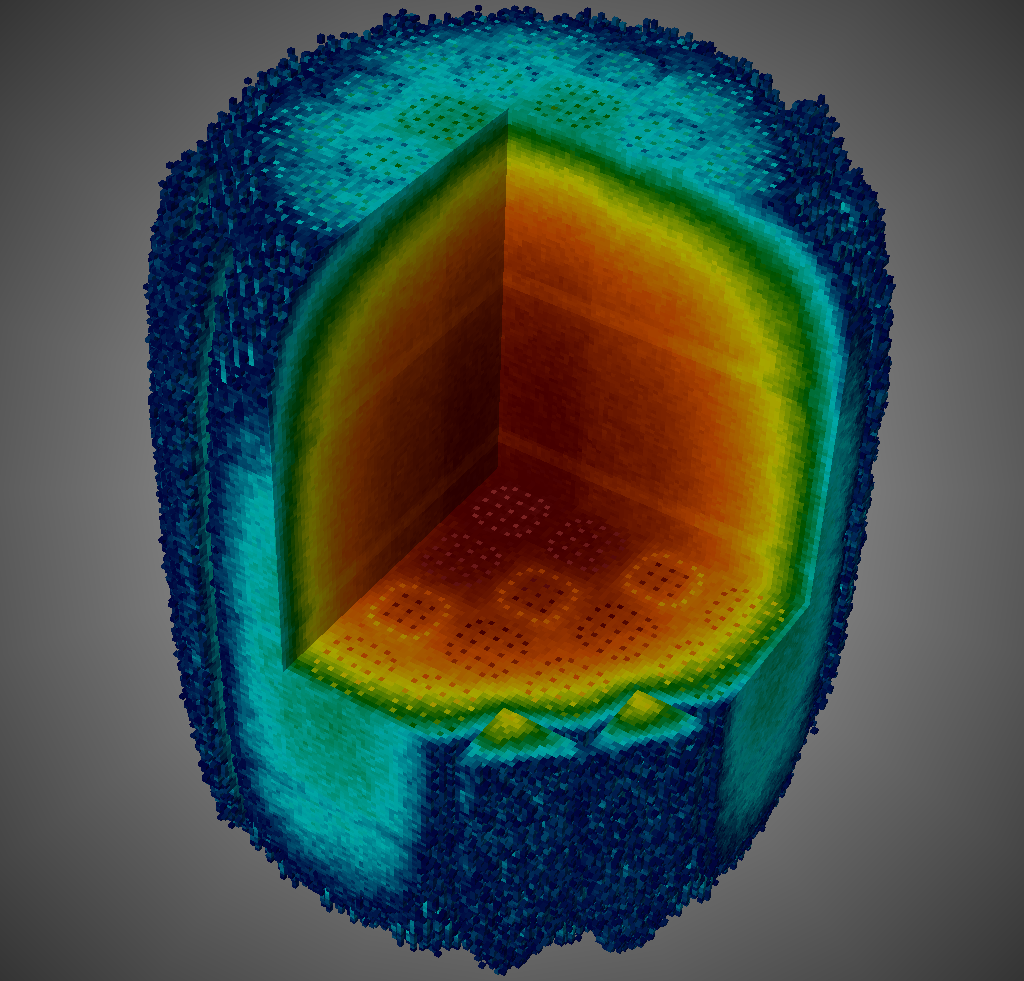
\includegraphics[width=2cm]{images/exasmr.png}
        \end{subfigure}
        \begin{subfigure}
           \centering
           
\includegraphics[width=2cm]{images/atr.png} 
        \end{subfigure}
        \begin{subfigure}
           \centering
           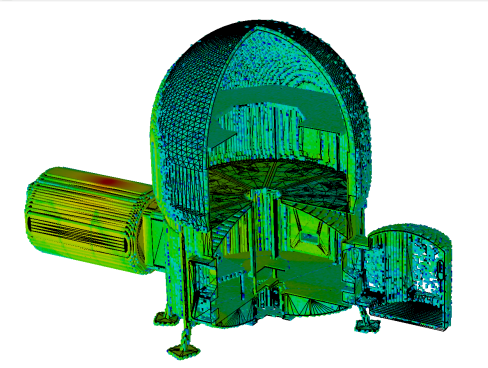
\includegraphics[width=2cm]{images/hab1.png} 
        \end{subfigure}
        \begin{subfigure}
            \centering
            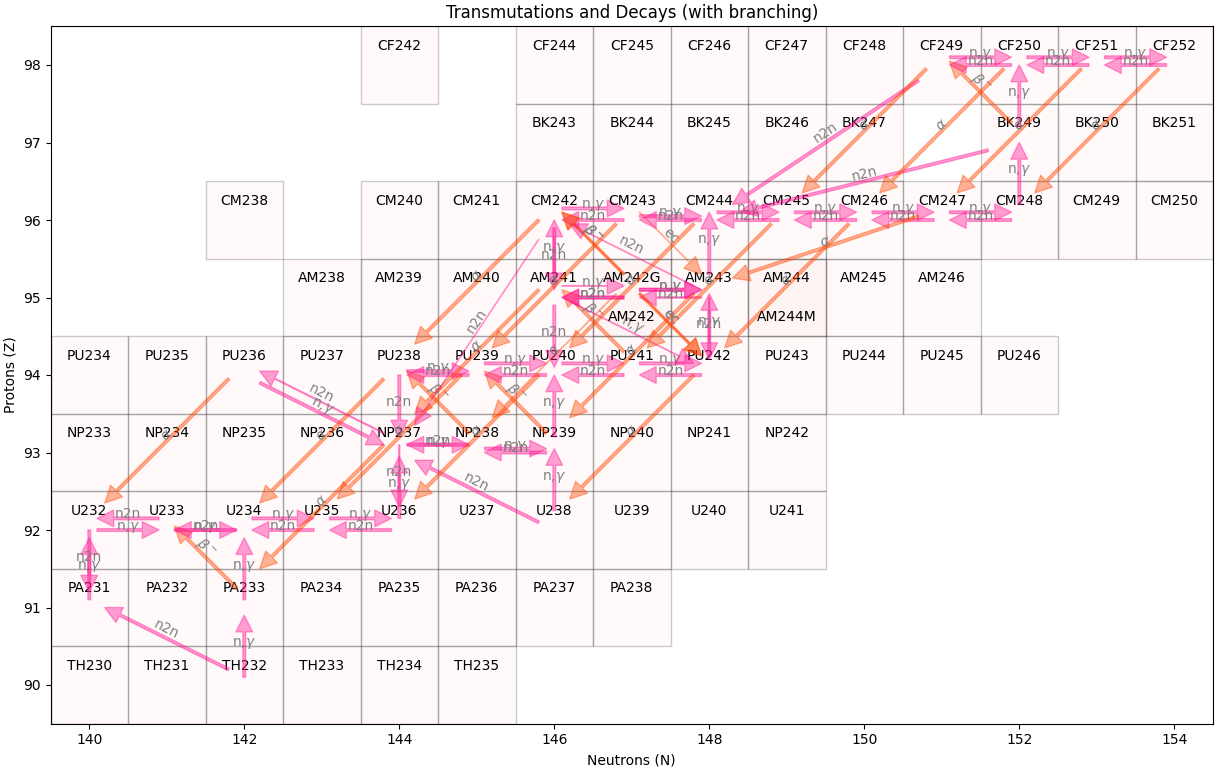
\includegraphics[width=4cm]{images/transmutation.png}
        \end{subfigure}
    \end{figure}
    \begin{center}
      {\tiny Sources: \cite{exasmr_fig},\cite{openmc_atr_slice},\cite{dagmc_nasa_module},\cite{armi_transmutation_fig}}
    \end{center}
    \pause\medskip
    \begin{itemize}
        \item Neutron transport
        \item Decay chains
        \item Materials
        \item Thermal hydraulics
        \item PRA
        \item Accident analysis
        \item {\bf Licensing activities}
    \end{itemize}

\end{frame}

\begin{frame}
    \frametitle{Open source software}
    Software whose source code is public.
    
    \begin{columns}
        \column[t]{5cm}
        \begin{itemize}
            \item Promotes collaborative contributions
            \item Reduces duplicate/competing work
        \end{itemize}

        \pause
        \column[t]{5cm}
        A sample of open-source codes in the nuclear space
        \begin{itemize}
            \item OpenMC (monte carlo neutron transport)
            \item MOOSE (multiphysics finite element framework)
            \item nekRS (Spectral element computational fluid dynamics)
        \end{itemize}
    \end{columns}
\end{frame}

\begin{frame}
    \frametitle{Open source advanced reactor modeling}
    Regulatory bodies will require new software features in order to effectively and efficiently perform licensing activities for the next generation of reactor designs\cite{usnrc_nonlwr_2020-1}
    \pause
    \newline
    \newline
    \Gls{IAEA} facilitated \Gls{ONCORE} initiative\cite{fiorina_initiative_2021}:
    \newline
    \newline
    \noindent ``ONCORE\ldots is an IAEA-facilitated international collaboration framework for the development and applictaion of open-source multi-physics simulation tools to support research, education, and training for analysis of advanced nuclear power reactors''\cite{iaea_open-source}
\end{frame}

\begin{frame}[t]
    \frametitle{How to develop features in open-source software?}

    There's no ``right'' way to do this, but there are useful conventions and concepts:
    \begin{itemize}
        \item Code standards (e.g. PEP8, The C Standard)
        \item User and developer guides
        \begin{itemize}
            \item Installation instructions
            \item API documentation
            \item Contributing guidelines
        \end{itemize}
        \item {\bf Version control}
        \item {\bf Open development}
        \item {\bf Automation}
    \end{itemize}
    These conventions and practices work in closed codes as well!
\end{frame}

\section{Useful practices}
\subsection{Version control}
\begin{frame}
  \frametitle{Document states}
  \begin{figure}[htpb]
      \centering
      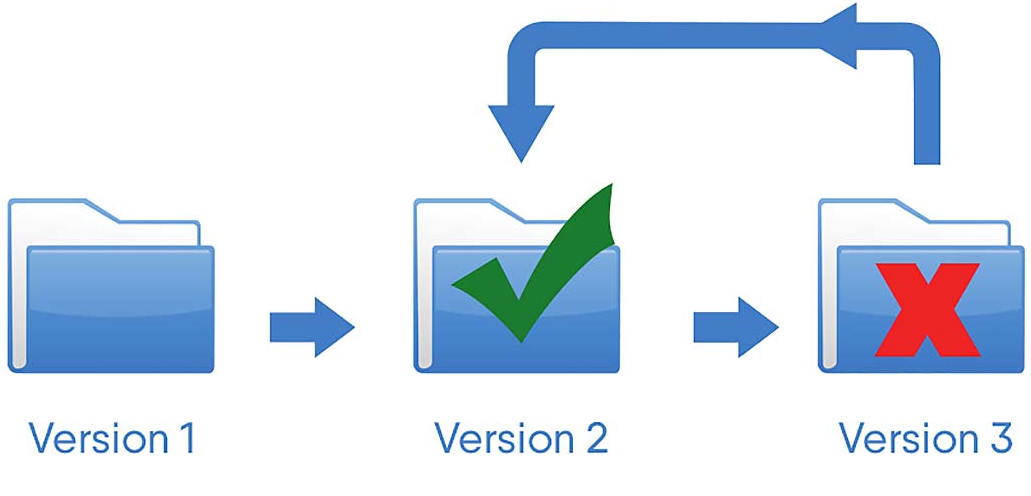
\includegraphics[width=0.8\textwidth]{images/singleton-vc.png}
  \end{figure}
\end{frame}

\begin{frame}
    \frametitle{Branching}
    \begin{figure}[htpb]
        \centering
        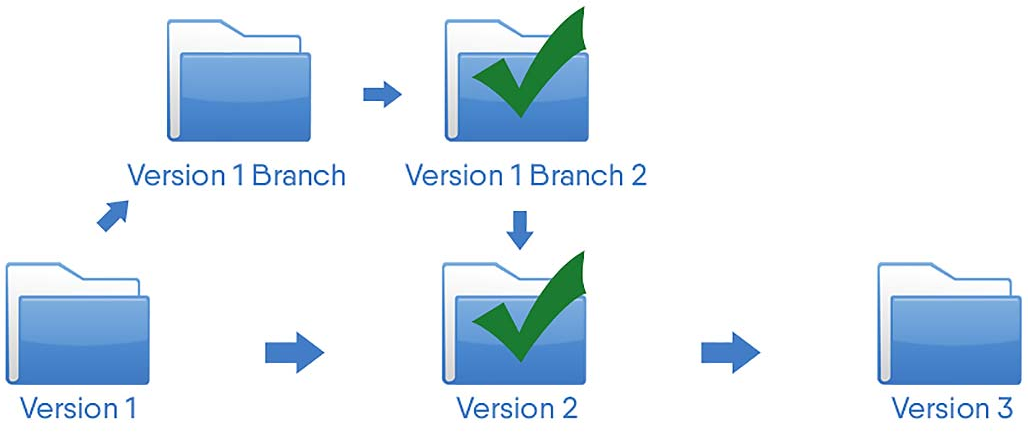
\includegraphics[width=0.8\textwidth]{images/branching-vc.png}
    \end{figure} 
\end{frame}

\begin{frame}
    \frametitle{Multiple branches}
    \ldots
    
\end{frame}

\subsection{Open development workflow}
\begin{frame}
  \frametitle{Open development: what is it?}
  \pause\medskip
  An answer:

  More than just hosting code publicly, it is a set of development practices that emphasizes reproducibility and searchability:
  \begin{itemize}
      \item Verbose commit messages
      \item Ticketing system to track bugs and feature proposals
      \item Robust justification for bug fixes and features
  \end{itemize}
  
  Web-based development platforms like GitHub, GitLab, and BitBucket all provide interfaces that can accomodate an open development approach. 
  \begin{figure}[htpb]
      \begin{subfigure}
          \centering
          
\includegraphics[width=1cm]{images/github-mark.eps}
      \end{subfigure}
      \begin{subfigure}
          \centering
          
\includegraphics[width=3cm]{images/gitlab-logo.eps}
      \end{subfigure}
      \begin{subfigure}
          \centering
          
\includegraphics[width=3cm]{images/bitbucket-logo.eps}
      \end{subfigure}
  \end{figure}
  \begin{center}
      {\tiny Sources: \cite{github_logo}, \cite{gitlab_logo}, \cite{bitbucket_logo}}
  \end{center}
\end{frame}

\begin{frame}
  \frametitle{Why open development?} 
  \begin{columns}
      \column[t]{5cm}
      Open development:
      \begin{itemize}
          \item creates developer-users $\rightarrow$ more robust code
          \item leverages the expertise of the community 
          \item \ldots 
      \end{itemize}

      Closed codes can adopt open development practices too!

      \column[t]{5cm}
      \begin{figure}[htpb]
          \centering
          
\includegraphics[width=2cm]{images/working-in-public.png}
      \end{figure}
      For more on open development, check out {\it Working in Public} by Nadia Eghbal \cite{eghbal_working_2020}

      
  \end{columns}
\end{frame}

\begin{frame}[fragile]
    \frametitle{Open development example}
    \framesubtitle{Implementing OpenMC in SaltProc}

    Idea: Implement OpenMC in an open-source Molten Salt Reactor depletion simulator\footnote{You can find the issue here: \url{https://github.com/arfc/saltproc/issues/133}} 
    \newline
    \newline
    In the issue tracker, I detail background/motivation and the description of the idea:


    \vspace{0.5cm}
    \begin{figure}[htpb]
        \centering
        
\includegraphics[width=10cm]{images/open-dev-ex1.png}
    \end{figure}

    
\end{frame}

\begin{frame}[fragile]
    \frametitle{Open development example}
    \framesubtitle{Implementing OpenMC in SaltProc}

    I also detail a skeleton design/implementation:


    \vspace{0.5cm}
    \begin{figure}[htpb]
        \centering
        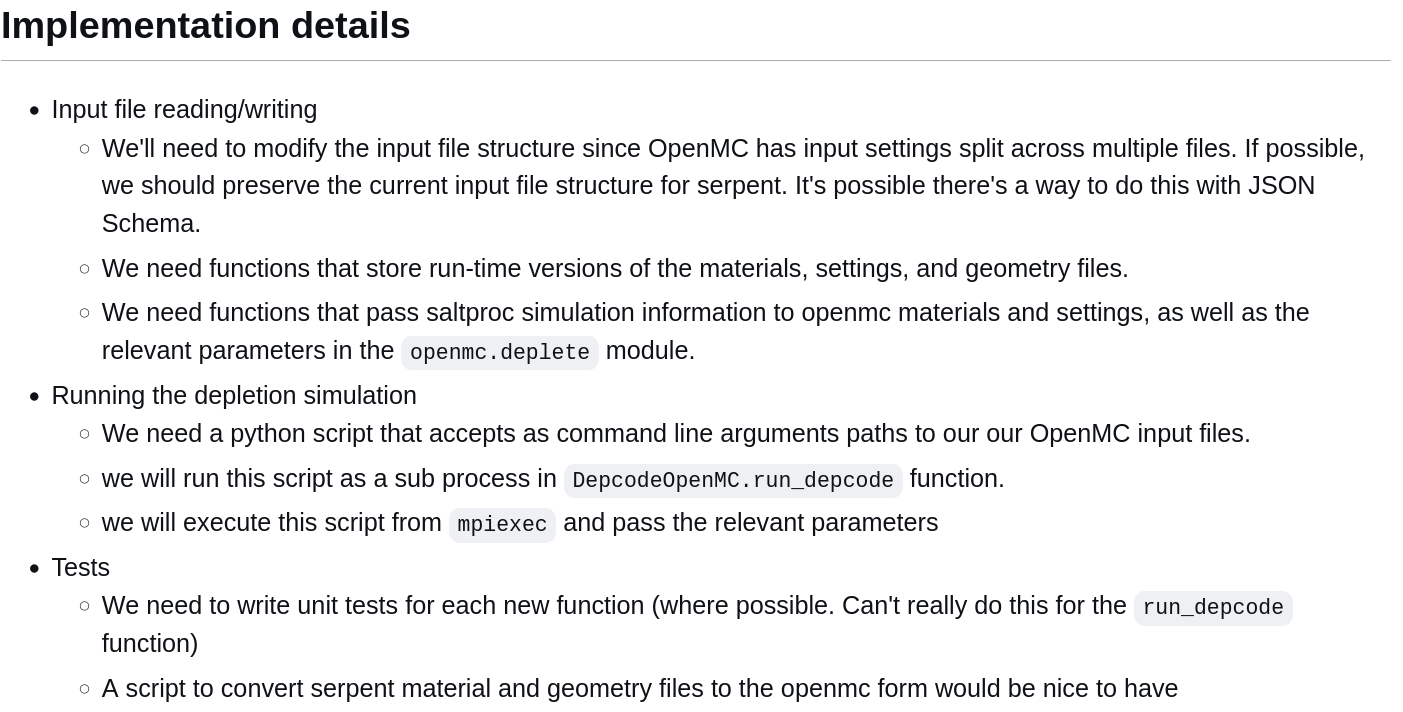
\includegraphics[width=10cm]{images/open-dev-ex2.png}
    \end{figure}

\end{frame}

\begin{frame}[fragile]
    \frametitle{Open development example}
    \framesubtitle{Implementing OpenMC in SaltProc}

    Finally, I write down any snags I can think of:
    \vspace{0.5cm}
    \begin{figure}[htpb]
        \centering
        
\includegraphics[width=10cm]{images/open-dev-ex3.png}
    \end{figure}

\end{frame}

\subsection{Automation and continuous integration}
\begin{frame}
  \frametitle{Intro to automation}
  \begin{figure}[htpb]
      \raggedleft
      
\includegraphics[width=2cm]{images/robot-icon.eps}
      \newline
      {\tiny Source: \cite{robot_icon}}
  \end{figure}

  Automating out\ldots

\end{frame}

\section{Conclusion}
\begin{frame}
    \frametitle{Main takeaways}
    \begin{itemize}
    \item Open source software is becoming more important in our field. 
    \pause
    \item Version control helps us keep track of changes and work on multiple features at once.
    \pause
    \item Open development ensures new and external contributors can understand design and implementation desicions.
    \pause
    \item Automating out repetitive tasks helps catch bugs and streamline the development workflow. 
    \end{itemize}
\end{frame}

\begin{frame}
  \frametitle{Acknowledgement}
        Acknowledgements should include both people who helped and funding 
        streams. If you are funded by an NEUP grant, that number usually goes 
        here. .
\end{frame}

%%--------------------------------%%
%%--------------------------------%%
\begin{frame}[allowframebreaks]
  \frametitle{References}
  \bibliographystyle{plain}
  {\footnotesize \bibliography{bibliography.bib} }

\end{frame}

%%--------------------------------%%


\end{document}



